\section{Scanning Methods}

An x-ray measurement always consists of an intensity measurement as a function of
the Euler-cradle movement. The intensity profile ideally consists of several
sharp peaks above a background. The width of the peaks is determined by the crystal
quality of the sample and is therefore of particular interest.

The Euler-cradle movement changes the scattering vector $\mathbf{q}$ as well as the
relative position of the laboratory coordinate system with respect to the reciprocal
crystal lattice, see [[XRD Coordinate Systems]].

Different constraints on the Euler-cradle motion lead to a variety of scanning
methods. Each has a different trajectory through the [[Ewald Sphere]] and therefore
reveals different information about the sample. Popular scanning methods are:

\subsection{Miscut Identification}\label{sec:miscut}

\begin{figure}
	\centering
	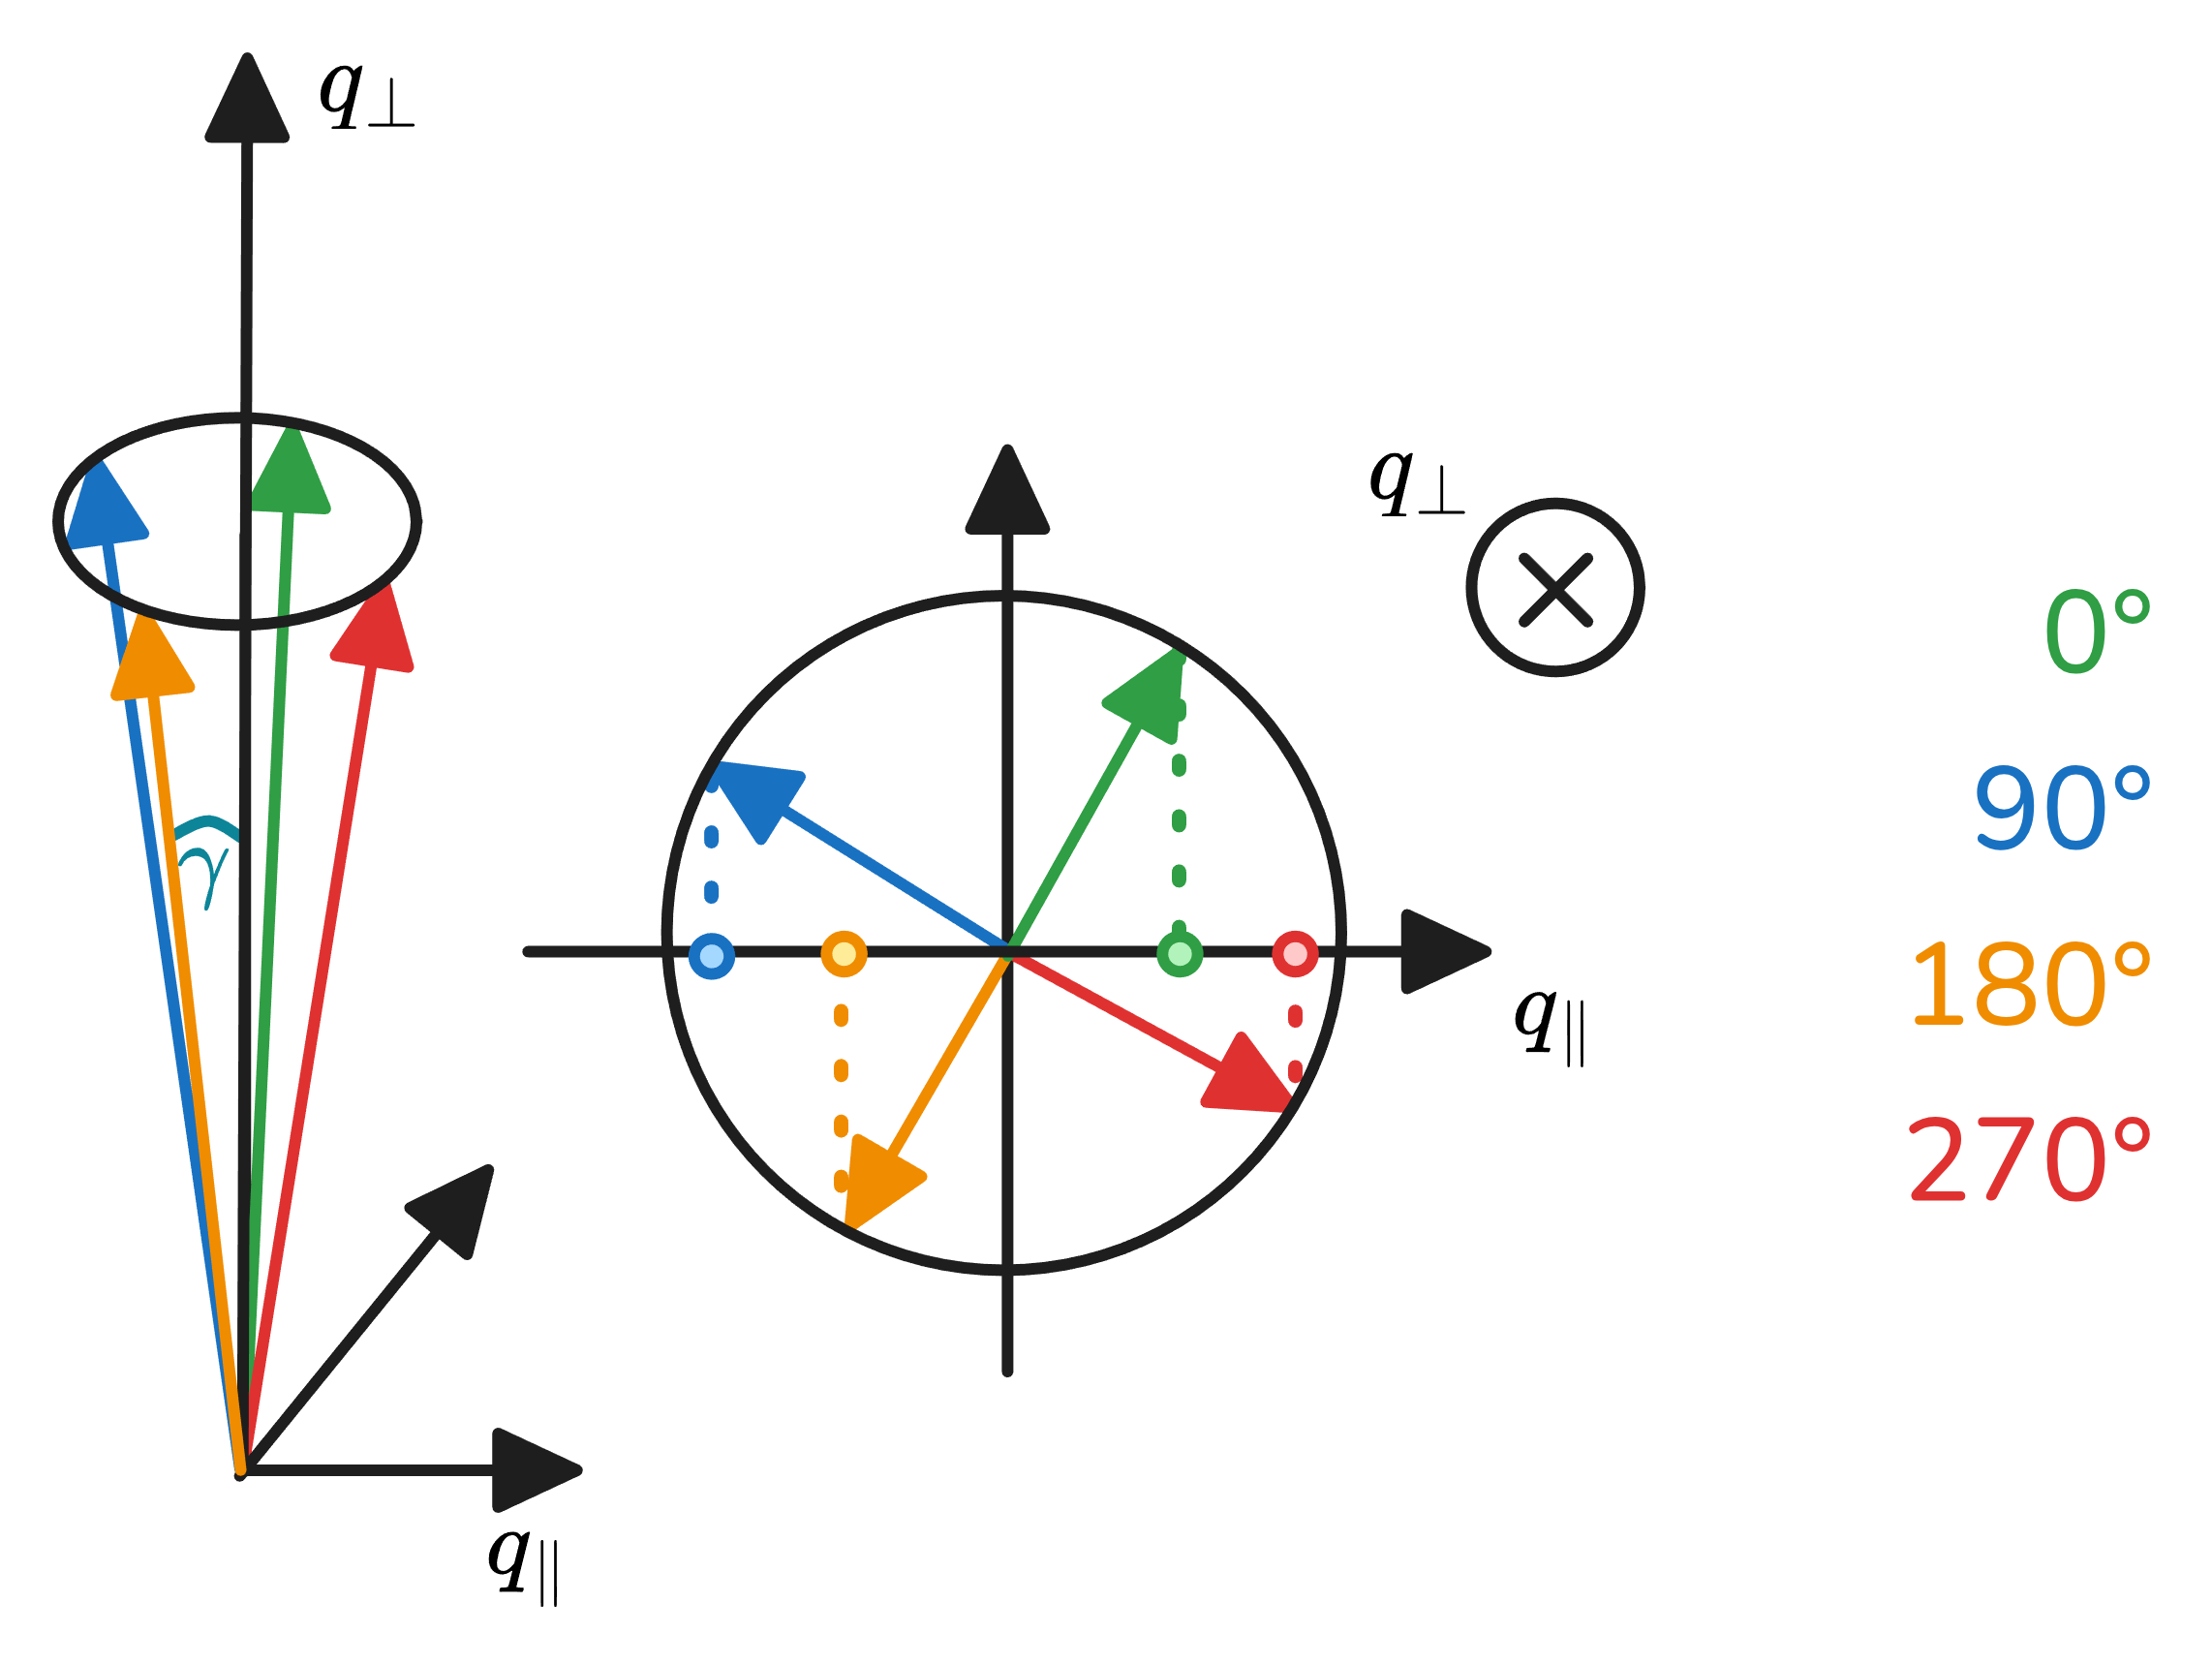
\includegraphics[width=0.8\textwidth]{../assets/scan_miscut.png}
	\caption{A miscut tilts the reciprocal-lattice vector $\mathbf{G}$ by the angle
		$\gamma$ out of the $\hat{q}_{\perp}$ direction. Rotating the sample about
		$\varphi$ sweeps the projection onto the scattering plane, which is measured
		at $\varphi = 0^\circ, 90^\circ, 180^\circ, 270^\circ$.}
	\label{fig:scan_miscut}
\end{figure}

An XRD instrument offers a very high resolution in the scattering plane, but a
lower resolution perpendicular to it. The axial acceptance describes the angular range,
out of the scattering plane, over which the diffractometer can still detect a reflection.
For those reflexes, the diffractometer effectively measures the projection onto the
scattering plane.

A symmetrical peak with miscut can be described with respect to the laboratory coordinate
system as:

\[
	\mathbf{G}=\lvert \mathbf{G}\rvert
	\begin{pmatrix}
		\sin(\gamma) \cos(\varphi+\varphi_{0}) \\
		\sin(\gamma) \sin(\varphi+\varphi_{0}) \\
		\cos(\gamma)
	\end{pmatrix}
\]

A perfectly aligned crystal features $\gamma =0$. Since the miscut is small, the reflex lies within the axial acceptance for all
$\varphi$. Therefore, the projection is measured as:

\[
	\begin{align}
		q_{\parallel} & =\lvert \mathbf{G}\rvert \sin(\gamma) \cos(\varphi+\varphi_{0}) \\
		q_{\perp}     & =\lvert \mathbf{G}\rvert \cos(\gamma)
	\end{align}
\]
Since the miscut is small, the length change of the projection is negligible. Therefore,
all reflexes are observed for a fixed $\theta_{\mathrm{B}}$. Using XRD Coordinate
Systems, a relation $\omega(\varphi)$ can be established to fit the data:

\[
	\omega-\theta_{\mathrm{B}}=\arctan\left( \frac{q_{\parallel}}{q_{\perp}}\right)
	=\arctan[\tan(\gamma)\cos(\varphi+\varphi_{0})] \\
\]
The paper defines the following helper angles, which are related to the miscut
angle $\gamma$ as:

\[
	\begin{align}
		\gamma_{0, 180}  & =\frac{1}{2}[(\omega_{0}-\theta_{\mathrm{B}})-(\omega_{180}-\theta_{\mathrm{B}})]=\arctan[\tan(\gamma) \cos(\varphi_{0})]   \\
		\gamma_{90, 270} & = \frac{1}{2}[(\omega_{270}-\theta_{\mathrm{B}})-(\omega_{90}-\theta_{\mathrm{B}})]=\arctan[\tan(\gamma) \sin(\varphi_{0})]
	\end{align}
\]
This yields the following identity:

\[
	\tan(\gamma_{0, 180})^{2}+\tan(\gamma_{90, 270})^{2}=\tan^{2}(\gamma)
\]
Using the small-angle approximation results in
$\gamma^{2}=\gamma_{0, 180}^{2}+\gamma_{90, 270}^{2}$.

\subsection{2TO Scans}

In a $2\theta\Omega$-scan, the sample is rotated around the $\Omega$-axis while
the detector rotates with twice the angular velocity, $\chi$ and $\varphi$ angles
are kept constant. This routine only \textbf{changes the magnitude} of the scattering
vector $\mathbf{q}$; its \textbf{direction remains constant}, since the
scattering vector is defined as (see XRD Coordinate Systems):

\[
	\mathbf{q}= 2k \sin(\theta)
	\begin{pmatrix}
		\sin(\Omega-\theta) \\
		\cos(\Omega-\theta)
	\end{pmatrix}
\]
\emph{Symmetrical reflexes} are reflexes that can be described by a reciprocal space
vector parallel to $\hat{q}_{\perp}$. By setting $\Omega=\theta$, these reflexes can
be observed.

\begin{figure}[H]
	\centering
	\begin{subfigure}[t]{0.55\linewidth}
		\centering
		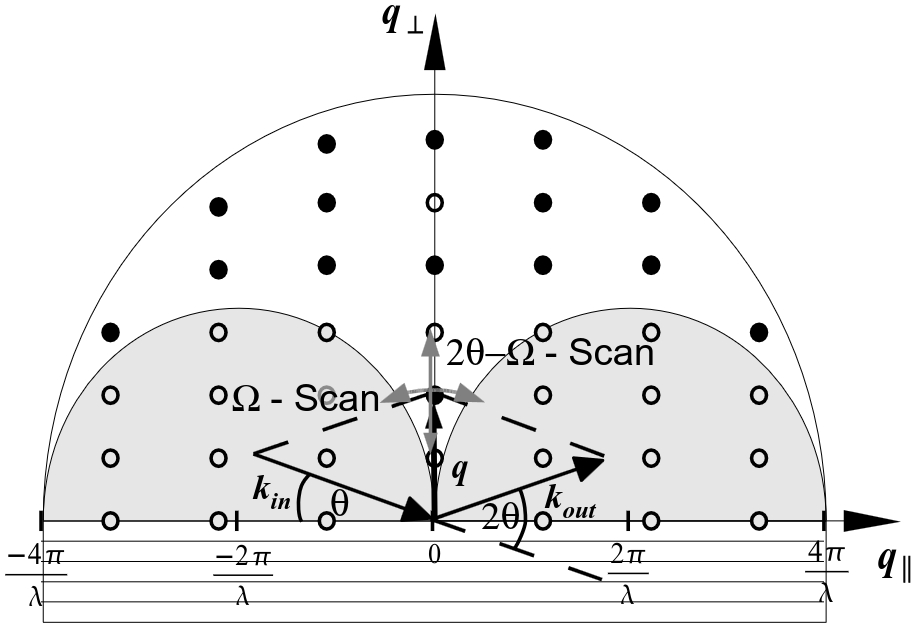
\includegraphics[width=\textwidth]{../assets/scan_2to.png}
		\caption{Trajectories through reciprocal space.}
		\label{fig:scan_2to}
	\end{subfigure}
	\hfill
	\begin{subfigure}[t]{0.35\linewidth}
		\centering
		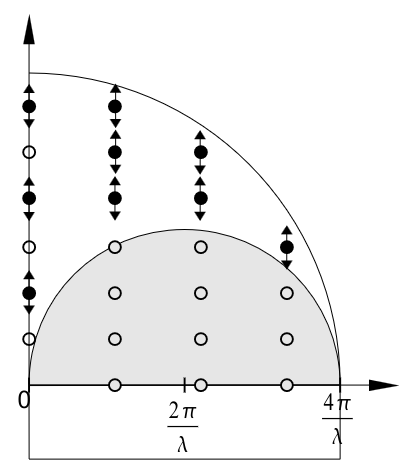
\includegraphics[width=\textwidth]{../assets/scan_2to_error.png}
		\caption{Peak broadening in $\hat{q}_{\perp}$ direction.}
		\label{fig:scan_2to_error}
	\end{subfigure}
	\caption{The $2\theta\Omega$-scan changes only the magnitude of the scattering
		vector $\mathbf{q}$, while its direction remains fixed.}
	\label{fig:scan_2to_full}
\end{figure}

Since thin films exhibit columnar growth, the vertical coherence length is not infinite
but limited by the layer thickness, which is around a couple of $\pu{ 100 nm}$. The
delta-distribution approximation in the $z$-direction of the intensity integral,
see Scattering intensity for periodic structures, does not hold. Therefore, the intensity
of a reflex broadens in $\hat{q}_{\perp}$ direction:

\[
	I(\mathbf{q}) \propto \left| \int_{V}\exp(\mathrm{i}(\mathbf{G}-\mathbf{q})\cdot
	\mathbf{r}) \, \mathrm{d}V(\mathbf{r}) \right|^{2}\simeq l_{x}l_{y}\delta(q_{x}
	, G_{x}) \delta(q_{y}, G_{y}) \left| \frac{\sin\left( l_{z}\frac{1}{2}(G_{z}-q_{z})
	\right)}{\frac{1}{2}(G_{z}-q_{z})}\right|^{2}
\]
\textbf{The FWHM of the reflex intensity correlates with the layer thickness}. If
other broadening effects are neglected, the thickness can be determined by the
following equation:

\[
	l_{z}=\frac{0.9 \lambda}{\Delta(2\theta) \cos(\theta)}
\]

Since the intensity distribution is determined by a sinc-function, secondary
maxima may be observed. The distance between secondary maxima is $\Delta q_{z}^{\mathrm{max}}
=\pi /l_{z}$. If $\Delta\theta$ denotes half the distance between secondary
maxima in a $2\theta\Omega$-scan, another equation related to the layer thickness
is:

\[
	l_{z}=\frac{\lambda \sin(\theta)}{\Delta\theta \sin(2\theta)}
\]

\subsection{Omega Scans}

In an $\Omega$-scan, the sample is rotated around the $\Omega$-axis, while
$\theta$, $\varphi$ and $\chi$ are kept constant. This routine moves the
scattering vector on a circular path around the origin (see XRD Coordinate Systems):

\[
	\mathbf{q}= 2k \sin(\theta)
	\begin{pmatrix}
		\sin(\Omega-\theta) \\
		\cos(\Omega-\theta)
	\end{pmatrix}
\]
\begin{figure}[H]
	\centering
	\begin{subfigure}[t]{0.45\linewidth}
		\centering
		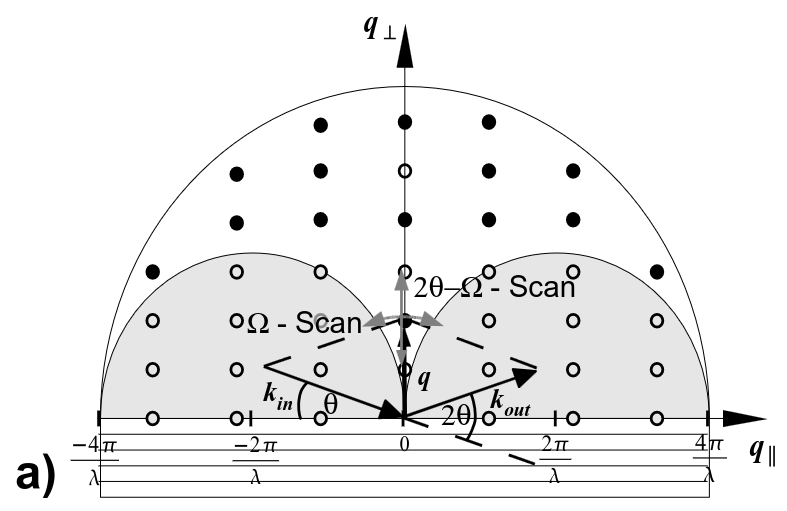
\includegraphics[width=\textwidth]{../assets/scan_omega.png}
		\caption{Trajectory through reciprocal space.}
		\label{fig:scan_omega}
	\end{subfigure}
	\hfill
	\begin{subfigure}[t]{0.5\linewidth}
		\centering
		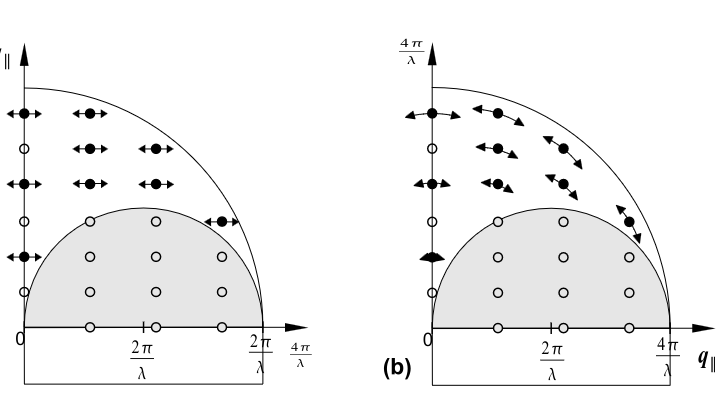
\includegraphics[width=\textwidth]{../assets/scan_omega_error.png}
		\caption{Peak broadening in $\hat{q}_{\parallel}$ direction.}
		\label{fig:scan_omega_error}
	\end{subfigure}
	\caption{The $\Omega$-scan moves the scattering vector $\mathbf{q}$ on a
		circular path around the origin.}
	\label{fig:scan_omega_full}
\end{figure}

\subsection{Peak Broadening}

\subsubsection{Lateral Coherence Length}

Due to the columnar growth mode, the lateral planes perpendicular to the $[001]$ direction
have a finite width (coherence length) for scattering limited by the crystallite size.
Similar to the discussion in 2TO-Scans, this leads to a peak broadening in $q_{\mathrm{\parallel}}$
direction. For a symmetrical rocking curve, assuming that the limited coherence size
is the only reason for peak broadening, the coherence length can be estimated as:

\begin{equation}
	L_{\parallel}=\frac{0.9 \lambda}{2\Delta\Omega\cdot \sin(\theta)}
	\label{eq:coherence_length}
\end{equation}
\subsubsection{Mosaicity}

Another broadening mechanism originates from the tilt of the crystallites. A
mosaic crystal is built up by many crystallites with tilt angles $\delta\Omega$. These
crystallites can be grouped into ensembles; rotating the sample around the
$\Omega$-axis selects different ensembles. The width of a symmetrical rocking curve
is therefore influenced by a \textbf{finite crystal size} and the \textbf{tilt
of crystallites}. The $\Delta\Omega_{002}$ becomes a figure of merit. The smaller
$\Delta\Omega_{002}$, the better the crystallites are aligned and the larger
their size.

![[Pasted image 20260616155141.png|500]]

\subsubsection{Crystallite Twist}

Since the twist of the crystallites has no influence on the $\Omega_{002}$
rocking curve, other peaks need to be included. Popular choices are the
$\{ 1 00 \}$-rocking curves that cannot be measured directly but have to be
interpolated from skew-geometry-measured $\{ h 0l \}$ peaks. A common approximation
is the $\{ 1 0 1 \}$ peak, which can be measured directly.

By assuming that broadening of rocking curves is only due to tilt and twist, it is
possible to calculate the dislocation densities with respect to the $[001]$-axis:

\begin{align}
	\rho_{\mathrm{screw}} & = \frac{\Delta\Omega_{002}^{2}}{4.35 \lvert \mathbf{b}_{\mathrm{screw}}\rvert^{2}} \label{eq:rho_screw} \\
	\rho_{\mathrm{edge}}  & =\frac{\Delta\Omega_{101}^{2}}{4.35 \lvert \mathbf{b}_{\mathrm{edge}}\rvert^{2}} \label{eq:rho_edge}
\end{align}
In this case $\mathbf{b}_{\mathrm{screw}}=\mathbf{b}_{3}$ and $\mathbf{b}_{\mathrm{edge}}
=1 /3 \cdot[ 110]a$.

\subsection{Reciprocal Space Maps}

A reciprocal space map scans a two-dimensional region of reciprocal space. The scan
can be carried out by repeating an $\Omega$-Scan for a fixed range followed by a tiny
shift using the $2\theta\Omega$ scan mode to change the length of the scattering vector.
The angles can be related to $q_{\parallel}$ and $q_{\perp}$ components via XRD
Coordinate Systems:

\[
	\mathbf{q}= 2k \sin(\theta)
	\begin{pmatrix}
		\sin(\Omega-\theta) \\
		\cos(\Omega-\theta)
	\end{pmatrix}
\]
The broadening mechanisms of finite coherence length, mosaicity and finite layer thickness
are visible. An RSM of an asymmetrical reflex allows the determination of $a$
and $c$ constants. Assume that $\hat{q}_{\parallel}$ is aligned with the $(100)$ direction
and $\hat{q}_{\perp}$ with $(001)$ direction. Peaks of the form $\{h\,0\,l\}$ can be
described by (see Hexagonal Lattice):

\[
	\begin{pmatrix}
		q_{\parallel} \\
		q_{\perp}
	\end{pmatrix}
	=
	\begin{pmatrix}
		h \cdot \frac{4\pi}{\sqrt{ 3 }a} \\
		l\cdot \frac{2\pi}{c}
	\end{pmatrix}
\]
$q_{\parallel /\perp}$ is usually given in relative units, i.e.
$q_{\mathrm{rlu}}=\lambda q /(4\pi)$